\begin{task}{Linear Regression}
In this exercise, we will implement various kinds of linear regression using the given data. For all subtasks, we assume that the data $(x_i, y_i)_{i \in \{1, \hdots, n \}}$ ($n$ is the number of points) is identically and independently distributed according to 
\begin{align*}
y_i = \Phi(x_i)^T w + \epsilon_i,
\end{align*}
where
\begin{align*}
\epsilon_i  \sim \mathcal{N} ( 0, \sigma^2 ),
\end{align*}
hence $\epsilon_i$ is normally distributed with mean $0$ and variance $\sigma^2$. The function $\Phi : \mathbb{R}^1 \to \mathbb{R}^n$ is a feature transformation such that
\begin{align*}
y \sim \mathcal{N} ( \Phi(X)^T w, \sigma^2 I).
\end{align*}
If no basis function is stated explicitely we use the data as is $\Phi(x) = x$. 
\begin{subtask}
In the following task we implement linear ridge regression using linear features, i.e. the data itself. We include an additional input dimension to represent a bias term and we use the ridge coefficient $\lambda = 0.01$.
\begin{enumerate}
\item It turns out that the classical linear regression is subject to overfitting if the number of attributes is relatively large compared to the number of training points. Christopher M. Bishop mentions in his book "Pattern Recognition and Machine Learning" that one technique that is often used to control the overfitting phenomenon in such cases is that of regularization, which involves adding a penalty term to the error function in order to discourage the coefficients from reaching large values. If we consider $\ell_2$-regularization we get the so-called ridge-regression model
\begin{align*}
w = \argmin_{w} \frac{1}{2} ||X^Tw - y||^2 + \frac{\lambda}{2} ||w||^2.
\end{align*}
The parameter $\lambda$ is then the ridge coefficient. If $\lambda$ is big, then we put more emphasis on getting small $w$ which means that we avoid overfitting. \\
Furthermore there exist a statistic argument for ridge regression. If we assume that 
\begin{align*}
P[y|x,w] \sim \mathcal{N}(y | w^T \phi(x), \sigma^2) \text{ and } w \sim \mathcal{N}(0 | \tau^2) \text{ independently}
\end{align*}
we can show that maximizing the likehood function is equivalent to minimize
\begin{align*}
w = \argmin_{w} \frac{1}{2} ||\hat{X}^Tw - y||^2 + \frac{\lambda}{2} ||w||^2.
\end{align*}
where $\hat{X}$ is our transformed data.
\item To derive the optimal model parameters by minimizing the squared loss function we use the solution formula on page 40.
\begin{align*}
w = (\hat{X} \hat{X}^T + \lambda I)^{-1} \hat{X} y 
\end{align*}
After implementation in python we get $w = \begin{pmatrix} -0.30946806  1.19109478 \end{pmatrix}$.
\item The root mean squared error of the train data is $0.41217801567361084$. The root mean squared error of the test data is $0.38428816992597875$.
\item The following plot shows the training data as black dots and the predicted function as a blue line. \\
\begin{center}
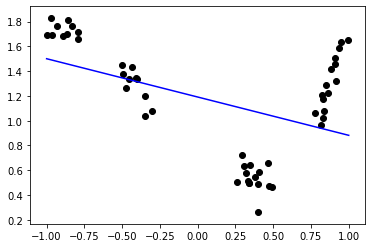
\includegraphics{Figure_1a.png}
\end{center}
Snippets of the code for 1a:
\begin{lstlisting}
def preprocess_X(X):
    ones_vector = np.ones(len(X))
    X_new = np.column_stack((X, ones_vector))
    return X_new.T

def lin_ridge_regression(X_train, y_train, lam):
    X_train_new = preprocess_X(X_train)
    x_x_T = np.matmul(X_train_new, X_train_new.T)
    I = np.eye(len(x_x_T))
    lambda_I = lam * I
    invers = np.linalg.inv(x_x_T + lambda_I)
    w = np.matmul(np.matmul(invers, X_train_new), y_train)
    return w

def solution_value(X, w):
    X_new = preprocess_X(X)
    return np.matmul(X_new.T,w)
    
def root_mean_squared_error(X_test ,w ,y_test):
    y_pred = solution_value(X_test, w)
    difference = np.linalg.norm(y_pred - y_test)/np.sqrt(len(y_pred))
    return difference
    
if __name__ == "__main__":
    # 1a
    w = lin_ridge_regression(lin_reg_train[:,0], lin_reg_train[:,1], 0.01)
    print("w linear ridge regression: ", w)
    y_pred = solution_value(lin_reg_test[:,0], w)
    
    difference_1a_train = root_mean_squared_error(lin_reg_train[:,0], w, lin_reg_train[:,1])
    print("Root mean squared error Train a", difference_1a_train)
    
    
    difference_1a_test = root_mean_squared_error(lin_reg_test[:,0], w, lin_reg_test[:,1])
    print("Root mean squared error Test a", difference_1a_test)
    
    #plot
    plt.scatter(lin_reg_train[:,0], lin_reg_train[:,1], c = "black")
    
    x = np.linspace(-1,1,100) # 100 linearly spaced numbers
    y_pred = solution_value(x,w)
    
    plt.plot(x,y_pred, c="blue")
    plt.show()
\end{lstlisting}
\end{enumerate}
\end{subtask}
\begin{subtask}
In this subtask we will implement linear ridge regression using a polynomial feature projection. We include an additional input dimension to represent a bias term and use the ridge coefficient $\lambda = 0.01$.
\begin{enumerate}
\item Polynomials of degree 2:
\begin{enumerate}
\item The root mean squared error of the training data is $0.21201447265968612$. The root mean squared error of the testing data is $0.21687242714148733$.
\item Single plot showing the training data as black dots and the predicted function as blue line:
\begin{center}
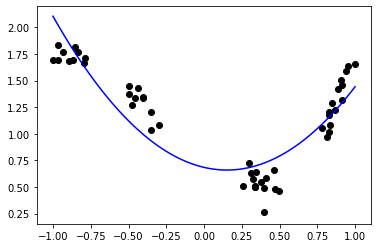
\includegraphics{Figure_1b_2.png}
\end{center}
\item One can combine linear regression with a nonlinear feature mapping to fit nonlinear function, i.e. we predict $w^T \phi(x)$ for some feature mapping $\phi : X \to \mathbb{R}^t$. The objective function that we want to fit stays $w^T x$. Hence the function that we want to fit is a nonlinear function of $x$,  but it is a linear function of the coefficients $w$. Hence this method is called \textit{linear} regression. 
\end{enumerate}
\item Polynomials of degree 3:
\begin{enumerate}
\item The root mean squared error of the training data is $0.0870682129548175$. The root mean squared error of the testing data is $0.10835803719738038$.
\item Single plot showing the training data as black dots and the predicted function as blue line:
\begin{center}
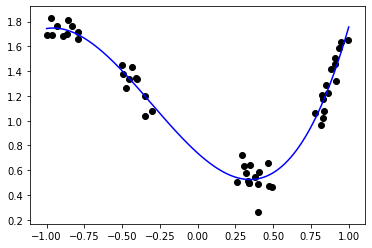
\includegraphics{Figure_1b_3.png}
\end{center}
\item See answer for degree 2.
\end{enumerate}
\item Polynomials of degree 4:
\begin{enumerate}
\item The root mean squared error of the training data is $0.08701261306638179$. The root mean squared error of the testing data is $0.10666239820964699$.
\item Single plot showing the training data as black dots and the predicted function as blue line:
\begin{center}
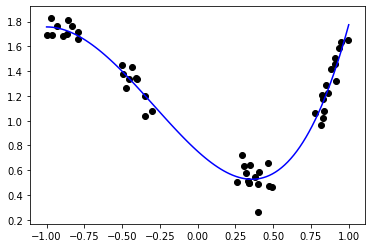
\includegraphics{Figure_1b_4.png}
\end{center}
\item See answer for degree 2.
\end{enumerate}
\end{enumerate}
Snippets of the code for 1b:
\begin{lstlisting}
def preprocess_X(X):
    ones_vector = np.ones(len(X))
    X_new = np.column_stack((X, ones_vector))
    return X_new.T

def lin_ridge_regression(X_train, y_train, lam):
    X_train_new = preprocess_X(X_train)
    x_x_T = np.matmul(X_train_new, X_train_new.T)
    I = np.eye(len(x_x_T))
    lambda_I = lam * I
    invers = np.linalg.inv(x_x_T + lambda_I)
    w = np.matmul(np.matmul(invers, X_train_new), y_train)
    return w

def solution_value(X, w):
    X_new = preprocess_X(X)
    return np.matmul(X_new.T,w)
    
def root_mean_squared_error(X_test ,w ,y_test):
    y_pred = solution_value(X_test, w)
    difference = np.linalg.norm(y_pred - y_test)/np.sqrt(len(y_pred))
    return difference

def stack(X_1, degree):
    X = X_1
    for i in range(2,degree+1):
        X = np.column_stack((X,np.power(X_1,i)))
    return X
    
#1b
    X_train = lin_reg_train[:,0]
    y_train = lin_reg_train[:,1]
    X_test = lin_reg_test[:,0]
    y_test = lin_reg_test[:,1]
    degree = 2
    
    X_train_new = stack(X_train, degree)
    w1 = lin_ridge_regression(X_train_new, y_train, 0.01)
    print("w linear ridge regression using a polynomial feature projection: ", w1)
    difference_1b_train = root_mean_squared_error(X_train_new, w1, y_train)
    print("Root mean squared error Train b ", difference_1b_train)
    
    X_test_new = stack(X_test, degree)
    difference_1b_test = root_mean_squared_error(X_test_new, w1, y_test)
    print("Root squared mean error Test b ", difference_1b_test)
    
    x = np.linspace(-1,1,100) # 100 linearly spaced numbers
    X_1 = stack(x, degree)
    y_pred = solution_value(X_1, w1)
    
    plt.scatter(lin_reg_train[:,0], lin_reg_train[:,1], c = "black")
    plt.plot(x,y_pred, c="blue")
    plt.show()

\end{lstlisting}
\end{subtask}
\begin{subtask}
In this subtask we implement 5-fold cross-validation to select the optimal degree for our polynomial degression.
\begin{enumerate}
\item Polynomial degree: $2$
\begin{enumerate}
\item Average train RMSE among all folds: $0.20943990135161356$
\item Average validation RMSE among all folds: $0.2248850559783977$
\item Average test RMSE among all folds: $0.21835094011192718$
\end{enumerate}
\item Polynomial degree: $3$
\begin{enumerate}
\item Average train RMSE among all folds: $0.08620813857069495$
\item Average validation RMSE among all folds: $0.09271100111785263$
\item Average test RMSE among all folds: $0.10927671570049995$
\end{enumerate}
\item Polynomial degree: $4$
\begin{enumerate}
\item Average train RMSE among all folds: $0.08547251620354353$
\item Average validation RMSE among all folds: $0.09841566883354039$
\item Average test RMSE among all folds: $0.10867173876433564$
\end{enumerate}
\item In the plots where the training data is shown as black dots one can cluster the points into 4 groups. At the beginning I thought that maybe the provided data is split in such a way that one group is in the validation set and the other groups are in the training set. In this situation, the cross-validation would perform very bad. \\
Since the training data is not ordered along the x-axis, the case described above did not happen. We excluded points from the training set that came from all groups. 
\item The polynomial degree 3 should be chosen, since the complexity of solving the system for polynomial degree 3 is less than for polynomial degree 4 and the polynomial with degree 4 does not perform much better than the polynomial with degree 3. Furthermore the polynomial of degree 3 performs better on the validation set then polynomial of degree 4. 
\end{enumerate}
Code snippets for 1c):
\begin{lstlisting}
def preprocess_X(X):
    ones_vector = np.ones(len(X))
    X_new = np.column_stack((X, ones_vector))
    return X_new.T

def lin_ridge_regression(X_train, y_train, lam):
    X_train_new = preprocess_X(X_train)
    x_x_T = np.matmul(X_train_new, X_train_new.T)
    I = np.eye(len(x_x_T))
    lambda_I = lam * I
    invers = np.linalg.inv(x_x_T + lambda_I)
    w = np.matmul(np.matmul(invers, X_train_new), y_train)
    return w

def solution_value(X, w):
    X_new = preprocess_X(X)
    return np.matmul(X_new.T,w)
    
    
def root_mean_squared_error(X_test ,w ,y_test):
    y_pred = solution_value(X_test, w)
    difference = np.linalg.norm(y_pred - y_test)/np.sqrt(len(y_pred))
    return difference

def stack(X_1, degree):
    X = X_1
    for i in range(2,degree+1):
        X = np.column_stack((X,np.power(X_1,i)))
    return X


def five_fold_cross_validation(train_data, test_data):
    X_1 = train_data[0:10]
    X_2 = train_data[10:20]
    X_3 = train_data[20:30]
    X_4 = train_data[30:40]
    X_5 = train_data[40:50]


    # Use subsets 1 - 4 to train your model with polynomial features of 
    degrees 2, 3 and 4.
    degrees = [2,3,4]
    subset_5 = [np.concatenate((X_1,X_2,X_3,X_4), axis = 0), X_5]
    subset_4 = [np.concatenate((X_1,X_2,X_3,X_5), axis = 0), X_4]
    subset_1 = [np.concatenate((X_2,X_3,X_4,X_5), axis = 0), X_1]
    subset_2 = [np.concatenate((X_3,X_4,X_5,X_1), axis = 0), X_2]
    subset_3 = [np.concatenate((X_4,X_5,X_1,X_2), axis = 0), X_3]
    
    
    
    
    subsets = [subset_1, subset_2, subset_3, subset_4, subset_5]
    

    for degree in degrees:
        RMSE_test = 0
        cross_RMSE_train = 0
        cross_RMSE_test = 0
        for subset in subsets:
            # define train and test set
            cross_validation_X_train = subset[0][:,0]
            cross_validation_y_train = subset[0][:,1]
            cross_validation_X_test = subset[1][:,0]
            cross_validation_y_test = subset[1][:,1]
            lam = 0.01
        
            
            cross_validation_X_train_new = stack(cross_validation_X_train, degree)
            
            w = lin_ridge_regression(cross_validation_X_train_new, cross_
            validation_y_train, lam)
            
            # RMSE for cross_validation
            cross_RMSE_train = cross_RMSE_train + root_mean_squared_error(cross_
            validation_X_train_new, w, cross_validation_y_train)
            
            cross_validation_X_test_new = stack(cross_validation_X_test, degree)
            
            cross_RMSE_test = cross_RMSE_test + root_mean_squared_error(cross_
            validation_X_test_new, w, cross_validation_y_test)
            
            #RMSE for test data
            X_test = test_data[:,0]
            y_test = test_data[:,1]
            
            X_test_new = stack(X_test, degree)
            
            RMSE_test = RMSE_test + root_mean_squared_error(X_test_new, w, y_test)
        print("degree: ", degree, "Average Train RMSE: ", cross_RMSE_train/5, 
        "Average Validation RMSE:", cross_RMSE_test/5, "Average Test RMSE: ", RMSE_test/5)
\end{lstlisting}
\end{subtask}
\begin{subtask}
In this subtask we implement Bayesian linear ridge regression, assuming that $w$ follows a multivariate Gaussian distribution, such that
\begin{align*}
w \sim \mathcal{N}(\mu_0, \Lambda_0^{-1})
\end{align*}
where ridge regression dictates $\mu_0 = 0$ and $\Lambda_0 = \lambda I$. \\
We assume $\sigma = 0.1$ and $\lambda = 0.01$ and include an additional input dimension to represent a bias term. We use all of the provided training data for a single Bayesian update. 
\begin{enumerate}
\item The posterior distribution of the model parameters $p(w | X,y)$ is
\begin{align*}
p(w|X,y) &= \mathcal{N}(\mu_n, \Lambda_n^{-1}) \\
\mu_n &= \Lambda_n^{-1}(\sigma^{-2} \Phi^Ty) \\
\Lambda_n &= \Lambda_0 + \sigma^{-2} \Phi^T \Phi %Siehe Bishop S.153
\end{align*}
\item Let $X_{*}$ be a batch of predictions. Then the predictive distribution is
\begin{align*}
p(y^{*}|X_{*}, X, y) &= \frac{1}{\sqrt{(2*\pi)^p \det(\Sigma)}} \exp (-\frac{1}{2} (y^*-\mu)^T \Sigma^{-1} (y^* - \mu)) \\
\mu(X_*) &= \phi(X_*) (\frac{\alpha}{\beta}I + \Phi \Phi^T)^{-1}\Phi^Ty \\
\Sigma &= \frac{1}{\beta} I + \phi^T(X_*)(\alpha I+ \beta \Phi \Phi^T)^{-1}\phi(X_*)
\end{align*}
\item The RMSE of the train data under our Bayesian model is: $0.41217792591659724$. The RMSE of the test data under our Bayesian model is: $0.38434085452132943$. 
\item The average log-likehood of the train data under our Bayesian model is: $-6.834699569913453$. The average log-likehood of the test data under our Bayesian model is: $-5.774748828572731$.
\item The following plot shows the training data as black dots, the mean of the predictive distribution as blue line and 1,2 and 3 standard deviations of the predictive distributions in shades of blue
\begin{center}
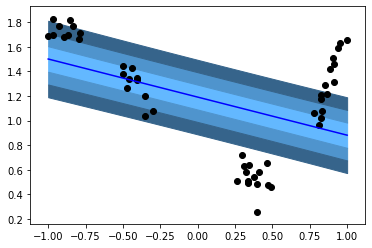
\includegraphics{Figure_1d.png}
\end{center}
\item The main difference between linear regression and Bayesian linear regression is that in linear regression we get an explicit $w$ such that the linear mapping $x^Tw$ describes our data well. In the case of Bayesian linear regression we get a predictive distribution which is Gaussian. The distribution depends on the noise of the data and the Gaussian prior of $w$. Furthermore the Bayesian treatment of linear regression will avoid over-fitting problem of the maximum-likehood and will also lead to automatic methods of determining model complexity using only the training data. (Bishop)
\end{enumerate}
Snippets of code for 1d):
\begin{lstlisting}
def preprocess_X(X):
    ones_vector = np.ones(len(X))
    X_new = np.column_stack((X, ones_vector))
    return X_new.T
    
def bayesian_linear_ridge_regression_mu(X,x,y):
    alpha = 0.01
    beta = 100
    
    X_new = preprocess_X(X)
    x_x_T = np.matmul(X_new, X_new.T)
    I = np.eye(len(x_x_T))
    lambda_I = (alpha/beta) * I
    invers = np.linalg.inv(x_x_T + lambda_I)
    w = np.matmul(np.matmul(invers, X_new), y_train)
    if type(x) != int:
        x_new = preprocess_X(x)
    else:
        x_new = np.asarray([x, 1])
    mu = np.matmul(x_new.T,w)
    return mu

def rmse_bayesian(X_train,y_train, data_set_x, data_set_y):
    y_pred = bayesian_linear_ridge_regression_mu(X_train, data_set_x, y_train)
    difference = np.linalg.norm(y_pred - data_set_y)/np.sqrt(len(y_pred))
    return difference

def log_likehood_bayesian(X_train, y_train, data_set_x, data_set_y, g=0, alpha=0.01, 
beta=100):
    
    average_log_likehood = 0
    
    mu = bayesian_linear_ridge_regression_mu(X_train, data_set_x, y_train)
    
    dev = np.zeros(len(mu))
    
    for i in range(len(data_set_x)):
        X_new = preprocess_X(X_train)
        x_x_T = np.matmul(X_new, X_new.T)
        I = np.eye(len(x_x_T))
        alpha_I = alpha * I
        beta_x_x_T = beta * x_x_T
        invers = np.linalg.inv(alpha_I + beta_x_x_T)
        if type(data_set_x[i]) == np.float64:
            data_set_x_new = np.append(data_set_x[i],1)
        else:
            data_set_x_new = preprocess_X(data_set_x[i].T)
        sigma_pre = np.matmul(np.matmul(data_set_x_new.T, invers),data_set_x_new)
        sigma = 1/beta + sigma_pre
        
        dev[i] = np.sqrt(sigma)

        # print("mu:", mu)
        # print("sigma", sigma)
        # print("x", data_set_x[i])
        # print("y", data_set_y[i])
        
        average_log_likehood = average_log_likehood + gaussian_density_function(mu[i], 
        sigma, data_set_y[i])

        
    if g==1:
        
        
        plt.plot(data_set_x, mu, c = "blue")
        plt.fill_between(data_set_x, mu, mu + dev, color='#63B8FF')
        plt.fill_between(data_set_x, mu, mu - dev, color='#63B8FF')
        plt.fill_between(data_set_x, mu + dev, mu + 2*dev, color='#4F94CD')
        plt.fill_between(data_set_x, mu - dev , mu - 2*dev, color='#4F94CD')
        plt.fill_between(data_set_x, mu + 2* dev, mu + 3*dev, color='#36648B')
        plt.fill_between(data_set_x, mu - 2*dev, mu - 3*dev, color='#36648B')
        
        plt.scatter(lin_reg_train[:,0], lin_reg_train[:,1], c = "black")
        plt.show()
    
    
        
    return average_log_likehood/len(data_set_x)
#1d
    
    X_train = lin_reg_train[:,0]
    y_train = lin_reg_train[:,1]
    X_test = lin_reg_test[:,0]
    y_test = lin_reg_test[:,1]
    
    bayesian_linear_ridge_regression_mu(X_train,[1, 2],y_train)
    
    # Report the RMSE of the train and test data under your Bayesian model 
    (use the predictive mean)
    
    print("RMSE Bayesian_training: ", rmse_bayesian(X_train,y_train, X_train, y_train))
    
    print("RMSE Bayesian Test: ",rmse_bayesian(X_train, y_train, X_test, y_test))
    
    # Report the average log-likelihood of the train and test data under your 
    Bayesian model.
    
    print("Log Likehood Train: ",log_likehood_bayesian(X_train, y_train, X_train, y_train))
    
    print("Log Likehood Test: ",log_likehood_bayesian(X_train, y_train, X_test, y_test))
    
    x = np.linspace(-1,1,100) # 100 linearly spaced numbers
    
    log_likehood_bayesian(X_train, y_train, x, y_test, g=1)
\end{lstlisting}
\end{subtask}
\begin{subtask}
In the following we implement Bayesian linear ridge regression using linear ridge regression model using squared exponential (SE) features. In other word, we replace our observed data matrix $X \in \mathbb{R}^{nx1}$ by a feature matrix $\Phi \in \mathbb{R}^{nxk}$, where
\begin{align*}
\Phi_{ij} = \exp(- \frac{1}{2} \beta (X_i - \alpha_j)^2).
\end{align*}
Set $k = 20$, $\alpha_j = j * 0.1 - 1$ and $\beta = 10$. We use the ridge coefficient $\lambda = 0.01$ and assume known Gaussian noise with $\sigma = 0.1$. We include an additional input dimension to represent a bias term. 
\begin{enumerate}
\item The RMSE of the train data under our Bayesian model with SE features is: $0.08160941530998907$. The RMSE of the test data under our Bayesian model with SE features is: $0.14341009681107458$.
\item The average log-likehood of the train data under our Bayesian model with SE feature is: $1.013494830677245$. The average log-likehood of the test data under our Bayesian model with SE feature is:
$0.5595070674582804$.
\item The following single plot show the training data as black dots, the mean of the predictive distribution as blue line and 1,2 and 3 standard deviations of the predictive distribution in shades of blue.
\begin{center}
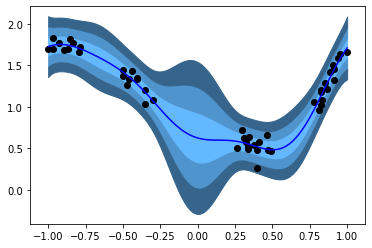
\includegraphics{Figure_1e.png}
\end{center}
\item 
\end{enumerate}
\begin{lstlisting}
def gaussian_density_function(mu, sigma, x):
    c1 = 1 / np.sqrt(2*np.pi * sigma)
    c2 = -0.5 * (x - mu)**2/ sigma
    y = np.log(c1) + c2
    return y    

def preprocess_X(X):
    ones_vector = np.ones(len(X))
    X_new = np.column_stack((X, ones_vector))
    return X_new.T
    
def bayesian_linear_ridge_regression_mu(X,x,y):
    alpha = 0.01
    beta = 100
    
    X_new = preprocess_X(X)
    x_x_T = np.matmul(X_new, X_new.T)
    I = np.eye(len(x_x_T))
    lambda_I = (alpha/beta) * I
    invers = np.linalg.inv(x_x_T + lambda_I)
    w = np.matmul(np.matmul(invers, X_new), y_train)
    if type(x) != int:
        x_new = preprocess_X(x)
    else:
        x_new = np.asarray([x, 1])
    mu = np.matmul(x_new.T,w)
    return mu

def rmse_bayesian(X_train,y_train, data_set_x, data_set_y):
    y_pred = bayesian_linear_ridge_regression_mu(X_train, data_set_x, y_train)
    difference = np.linalg.norm(y_pred - data_set_y)/np.sqrt(len(y_pred))
    return difference
    
def log_likehood_bayesian_SE(X_train, y_train, data_set_x, data_set_y, data_set_x_pre, 
g=0, alpha=0.01, beta=100):
    
    average_log_likehood = 0
    
    mu = bayesian_linear_ridge_regression_mu(X_train, data_set_x, y_train)
    
    dev = np.zeros(len(mu))
    
    for i in range(len(data_set_x)):
        X_new = preprocess_X(X_train)
        x_x_T = np.matmul(X_new, X_new.T)
        I = np.eye(len(x_x_T))
        alpha_I = alpha * I
        beta_x_x_T = beta * x_x_T
        invers = np.linalg.inv(alpha_I + beta_x_x_T)
        if type(data_set_x[i]) == np.float64 or len(data_set_x[i] == 1):
            data_set_x_new = np.append(data_set_x[i],1)
        else:
            data_set_x_new = preprocess_X(data_set_x[i].T)
        sigma_pre = np.matmul(np.matmul(data_set_x_new.T, invers),data_set_x_new)
        sigma = 1/beta + sigma_pre
        
        dev[i] = np.sqrt(sigma)

        # print("mu:", mu)
        # print("sigma", sigma)
        # print("x", data_set_x[i])
        # print("y", data_set_y[i])
        
        
        average_log_likehood = average_log_likehood + gaussian_density_function(mu[i], 
        sigma, data_set_y[i])
        
    if g == 1:
    
    
    
        plt.plot(data_set_x_pre, mu, c = "blue")
        plt.fill_between(data_set_x_pre, mu, mu + dev, color='#63B8FF')
        plt.fill_between(data_set_x_pre, mu, mu - dev, color='#63B8FF')
        plt.fill_between(data_set_x_pre, mu + dev, mu + 2*dev, color='#4F94CD')
        plt.fill_between(data_set_x_pre, mu - dev , mu - 2*dev, color='#4F94CD')
        plt.fill_between(data_set_x_pre, mu + 2* dev, mu + 3*dev, color='#36648B')
        plt.fill_between(data_set_x_pre, mu - 2*dev, mu - 3*dev, color='#36648B')
        
        plt.scatter(lin_reg_train[:,0], lin_reg_train[:,1], c = "black")
        plt.show()
    
    
        
    return average_log_likehood/len(data_set_x)

def feature_mapping(X,k, beta):
    PHI_pre = np.zeros((len(X),k))
    for i in range(len(X)):
        for j in range(k):
            alpha_j = (j+1) * 0.1 - 1
            PHI_pre[i,j] = np.exp(-0.5 * beta * (X[i] - alpha_j)**2)
    return PHI_pre
    
    
 #1e
    
    k = 20
    beta = 10
    PHI = feature_mapping(X_train,k, beta) # vorsicht! samples in den zeilen

    PHI_test = feature_mapping(X_test,k, beta)

    
    # # Report the RMSE of the train and test data under your Bayesian model with SE features
    
    print("RMSE Bayesian_SE_training: ", rmse_bayesian(PHI ,y_train, PHI, y_train))
    
    print("RMSE Bayesian_SE Test: ",rmse_bayesian(PHI, y_train, PHI_test, y_test))
    
    # # Report the average log-likelihood of the train and test data under your Bayesian model.
    
    
    print("Average Log Likehood SE Train: ",log_likehood_bayesian_SE(PHI, y_train, 
    PHI, y_train, X_train))
    
    print("Average Log Likehood SE Test: ",log_likehood_bayesian_SE(PHI, y_train, 
    PHI_test, y_test, X_test))
    
    # Real Plot
    
    x = np.linspace(-1,1,100) # 100 linearly spaced numbers
    
    X = feature_mapping(x,k, beta)
    
    g=1
    
    log_likehood_bayesian_SE(PHI, y_train, X, y_test, x, g)
\end{lstlisting}
\end{subtask}
\end{task}

\begin{task}{Statistics Refresher}
\begin{subtask}
Solution
\end{subtask}
\begin{subtask}
Solution
\end{subtask}
\begin{subtask}
Solution
\end{subtask}
\end{task}

\begin{task}{Optimization and Information Theory}
\begin{subtask}
Solution
\end{subtask}
\begin{subtask}
Solution
\end{subtask}
\begin{subtask}
Solution
\end{subtask}
\begin{subtask}
Solution
\end{subtask}
\end{task}